%% bare_jrnl_compsoc.tex
%% V1.4a
%% 2014/09/17
%% by Michael Shell
%% See:
%% http://www.michaelshell.org/
%% for current contact information.
%%
%% This is a skeleton file demonstrating the use of IEEEtran.cls
%% (requires IEEEtran.cls version 1.8a or later) with an IEEE
%% Computer Society journal paper.
%%
%% Support sites:
%% http://www.michaelshell.org/tex/ieeetran/
%% http://www.ctan.org/tex-archive/macros/latex/contrib/IEEEtran/
%% and
%% http://www.ieee.org/

%%*************************************************************************
%% Legal Notice:
%% This code is offered as-is without any warranty either expressed or
%% implied; without even the implied warranty of MERCHANTABILITY or
%% FITNESS FOR A PARTICULAR PURPOSE! 
%% User assumes all risk.
%% In no event shall IEEE or any contributor to this code be liable for
%% any damages or losses, including, but not limited to, incidental,
%% consequential, or any other damages, resulting from the use or misuse
%% of any information contained here.
%%
%% All comments are the opinions of their respective authors and are not
%% necessarily endorsed by the IEEE.
%%
%% This work is distributed under the LaTeX Project Public License (LPPL)
%% ( http://www.latex-project.org/ ) version 1.3, and may be freely used,
%% distributed and modified. A copy of the LPPL, version 1.3, is included
%% in the base LaTeX documentation of all distributions of LaTeX released
%% 2003/12/01 or later.
%% Retain all contribution notices and credits.
%% ** Modified files should be clearly indicated as such, including  **
%% ** renaming them and changing author support contact information. **
%%
%% File list of work: IEEEtran.cls, IEEEtran_HOWTO.pdf, bare_adv.tex,
%%                    bare_conf.tex, bare_jrnl.tex, bare_conf_compsoc.tex,
%%                    bare_jrnl_compsoc.tex, bare_jrnl_transmag.tex
%%*************************************************************************


% *** Authors should verify (and, if needed, correct) their LaTeX system  ***
% *** with the testflow diagnostic prior to trusting their LaTeX platform ***
% *** with production work. IEEE's font choices and paper sizes can       ***
% *** trigger bugs that do not appear when using other class files.       ***                          ***
% The testflow support page is at:
% http://www.michaelshell.org/tex/testflow/


\documentclass[10pt,conference,onecolumn,compsoc]{IEEEtran}


\usepackage{hyperref}
\usepackage{enumitem}
\setlist[itemize]{leftmargin=3 cm}
\setlist[enumerate]{leftmargin=3cm}



% *** CITATION PACKAGES ***
%
\ifCLASSOPTIONcompsoc
  % IEEE Computer Society needs nocompress option
  % requires cite.sty v4.0 or later (November 2003)
  \usepackage[nocompress]{cite}
\else
  % normal IEEE
  \usepackage{cite}
\fi
% cite.sty was written by Donald Arseneau
% V1.6 and later of IEEEtran pre-defines the format of the cite.sty package
% \cite{} output to follow that of IEEE. Loading the cite package will
% result in citation numbers being automatically sorted and properly
% "compressed/ranged". e.g., [1], [9], [2], [7], [5], [6] without using
% cite.sty will become [1], [2], [5]--[7], [9] using cite.sty. cite.sty's
% \cite will automatically add leading space, if needed. Use cite.sty's
% noadjust option (cite.sty V3.8 and later) if you want to turn this off
% such as if a citation ever needs to be enclosed in parenthesis.
% cite.sty is already installed on most LaTeX systems. Be sure and use
% version 5.0 (2009-03-20) and later if using hyperref.sty.
% The latest version can be obtained at:
% http://www.ctan.org/tex-archive/macros/latex/contrib/cite/
% The documentation is contained in the cite.sty file itself.



% *** GRAPHICS RELATED PACKAGES ***
%
\ifCLASSINFOpdf
   \usepackage[pdftex]{graphicx}
 
\else
 
\fi
% graphicx was written by David Carlisle and Sebastian Rahtz. It is
% required if you want graphics, photos, etc. graphicx.sty is already
% installed on most LaTeX systems. The latest version and documentation
% can be obtained at: 
% http://www.ctan.org/tex-archive/macros/latex/required/graphics/
% Another good source of documentation is "Using Imported Graphics in
% LaTeX2e" by Keith Reckdahl which can be found at:
% http://www.ctan.org/tex-archive/info/epslatex/
%
% latex, and pdflatex in dvi mode, support graphics in encapsulated
% postscript (.eps) format. pdflatex in pdf mode supports graphics
% in .pdf, .jpeg, .png and .mps (metapost) formats. Users should ensure
% that all non-photo figures use a vector format (.eps, .pdf, .mps) and
% not a bitmapped formats (.jpeg, .png). IEEE frowns on bitmapped formats
% which can result in "jaggedy"/blurry rendering of lines and letters as
% well as large increases in file sizes.
%
% You can find documentation about the pdfTeX application at:
% http://www.tug.org/applications/pdftex









% *** PDF, URL AND HYPERLINK PACKAGES ***
%
\usepackage{url}
% url.sty was written by Donald Arseneau. It provides better support for
% handling and breaking URLs. url.sty is already installed on most LaTeX
% systems. The latest version and documentation can be obtained at:
% http://www.ctan.org/tex-archive/macros/latex/contrib/url/
% Basically, \url{my_url_here}.




\begin{document}

\title{Spitfire '91, a WPF Shmup}
%
%

% received ..."  text while in non-compsoc journals this is reversed. Sigh.

\author{Victor Gasior and Jaxx Woods
}

\IEEEtitleabstractindextext{%
\begin{abstract}
Spitfire '91 is a retro inspired Shoot 'em Up game (or shmup) where you control a small airplane fighting enemy aircraft. The target audience for this project is fans of retro schups like EDF or UN Squadron.
\end{abstract}

}


% make the title area
\maketitle



\IEEEdisplaynontitleabstractindextext

\IEEEpeerreviewmaketitle



\section{Introduction}
Spitfire '91 is a fun, fast paced, retro inspired Shoot 'em Up game made in WPF / C Sharp. In Spitfire '91 the player controls a modern military fighter jet and fights enemy jets (repersented by colored squares). The game is designed to emulate an SNES (Super Nintendo Entertainment System) era Shoot 'em Up game with its own art, design, sounds, and mechanics. There is one stage where the players can fight enemies until they die in order to try to get a higher and higher high scores. The target audience for this game will be Shoot 'em Up enthusiasts and fans of retro styled video games in general. The audience should first and foremost enjoy the game, while also tailoring the experience to resemble a retro Shoot 'em Up without making it difficult for fans of modern video games to enjoy.  There are not many Shoot 'em Up games produced any more so we are appealing to a niche audience starved of content.

% needed in second column of first page if using \IEEEpubid
%\IEEEpubidadjcol


\subsection{Background}
Shoot em' Ups rely on a player controlled vehicle that can move around the screen and shoot enemies that are trying to attack the player. The player obtains points by avoiding and defeating enemies. The game ends once they reach the end of the level / stage or loses do to being hit by enemies too many times, some Shoot 'em Ups are endless where a player goes for a highscore, like Galaga.

The reason we decided to undertake this project is that Shoot 'em Ups are both fun to play, and seem interesting to design.

\subsubsection{Important Terminology}
\begin{itemize}
\item Shump - Common abbreviation for Shoot 'em Up
\item High Score - A goal of a Shoot 'em Up game, players try to earn higher scores.
\item Collision - How the game detects whether or not a game object has toutched another game object.
\end{itemize}

\subsection{Impacts}
This game should bring enjoyment to the audience and provide a free, modern alternative to old retro Shoot 'em Up games that can be hard to play due to old hardware and games not being ported to modern systems.

\subsection{Challenges}
Core game functions like handling enemy, projectile, and player collision in WPF. Normally we would use a dedicated game engine like Godot or Unity, but due to the requirements of this project, we must make these functions ourself in WPF.


\section{Scope}
This game contains one playable level with multiple enemy variations that can spawn. This level is infinite and goes until the player loses, like Galaga. There will be a win and lose state, as well as a connected lose state screen on loss. There will be a main menu screen the user accesses first before starting the main game. There will be a high score tracker which displays and saves the highest scores to add replay value. Current Stretch Goals are as follows: multiple levels with different backgrounds, a working upgrade shop and currency system, and music. Music is currently completed, as it was very quick and easy. With the upgrade shop players can use some of their score (the curreny) to purchase upgrades for their ship.

\subsection{Requirements}
We developed our requirements based on what we think will be the most fun for the user to experience. The requirements both make it so the game is operational (i.e. game actually works, core elements, etc. ), while also trying to make the user experience as great as possible (i.e. sound and visual effect feedback).

\subsubsection{Functional}
\begin{itemize}
\item User needs to be able to control the character to avoid enemies and shoot enemies.
\item User needs to be able to earn points by eliminating enemies.
\item User needs to be able to view their current score.
\item Game needs to spawn enemies for the player to both avoid and shoot.
\item User needs to be able to lose.
\item There should be visual effects and sound effects to enhance the game experience.
\item There should be a scrolling background to give the user the impression of flying
\end{itemize}

\subsubsection{Non-Functional}
\begin{itemize}
\item High scores will be persistenty stored between runs
\item Custom keybinidng (such as changing movement from arrow keys to WASD)
\item Enemy randomization for replayability
\end{itemize}

\subsection{Use Cases}
 \ref{tab:useCaseIndex}.




\begin{table}
\centering
\begin{tabular}{|c|c|c|c|c|}
\hline
Use Case ID & Use Case Name & Primary Actor & Complexity & Priority \\
\hline \hline
1 & Play Game & user & High & 1\\
\hline
2 & Check Highscore & user & Med & 2\\
\hline
3 & Pause Game & user & Easy & 3\\
\hline
\end{tabular}
\caption{Sample use case table}
\label{tab:useCaseIndex}
\end{table}


\begin{itemize}
\item[Use Case Number:] 1
\item[Use Case Name:] Playing the Game
\item[Description:] A user wants to play the game.
\end{itemize}

\begin{enumerate}
\item User opens the application.
\item User hits play.
\item User plays the game until loss.
\item[Termination Outcome:] The user's score is saved, highest score is updated if this score is the new highest score, which is displayed on the main menu. 
\end{enumerate}

\begin{itemize}
\item[Use Case Number:] 2
\item[Use Case Name:] Check Highscore
\item[Description:] A user wants to check the highscore of the local game.
\end{itemize}

\begin{enumerate}
\item User opens the application.
\item[Termination Outcome:] The user looks at the score on the main menu. If they are midgame they can look at the top right corner of the screen where the current score is displayed.
\end{enumerate}


\begin{itemize}
\item[Use Case Number:] 3
\item[Use Case Name:] Pausing the Game
\item[Description:] A user wants to pause the game during use
\end{itemize}

\begin{enumerate}
\item User is currently playing the game.
\item User pauses the game using the p key
\item[Termination Outcome:] The user keeps the game paused for as long as they want, unpausing if they wish by hitting p again
\end{enumerate}


\subsection{Interface}
Since we did not get to making the Interface elements such as the Game Over Screen and Main Menu in this version of the project, included are the mockups for them in the interface section.

\begin{figure}[ht!]
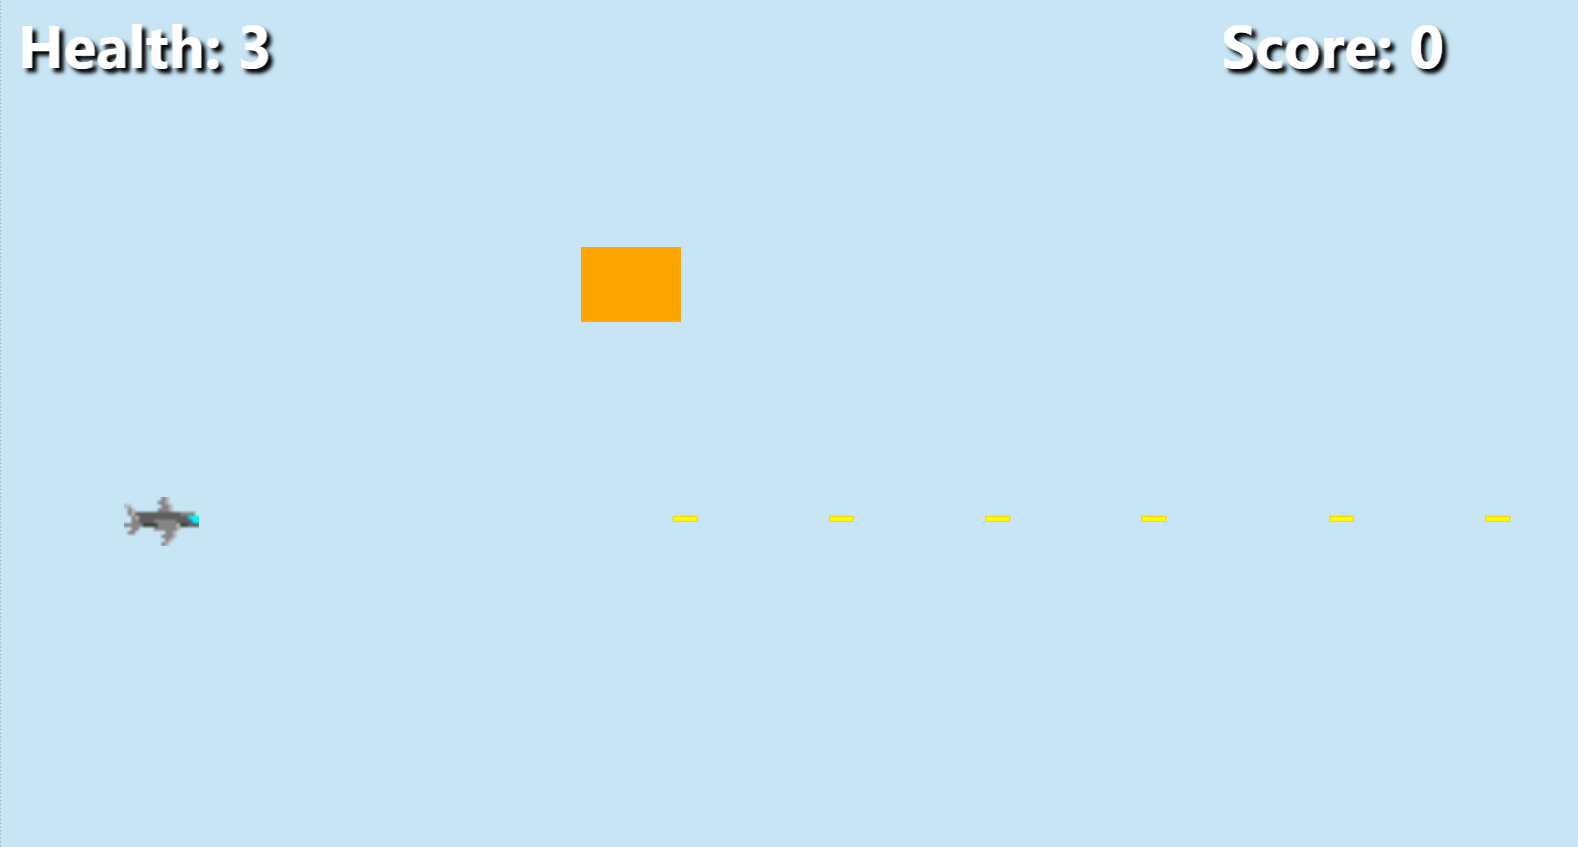
\includegraphics[height=250px, width=350px]{GAMEACTION.png}
\caption{This displays how the game looks during play}
\label{gameplay}
\end{figure}

\begin{figure}[ht!]
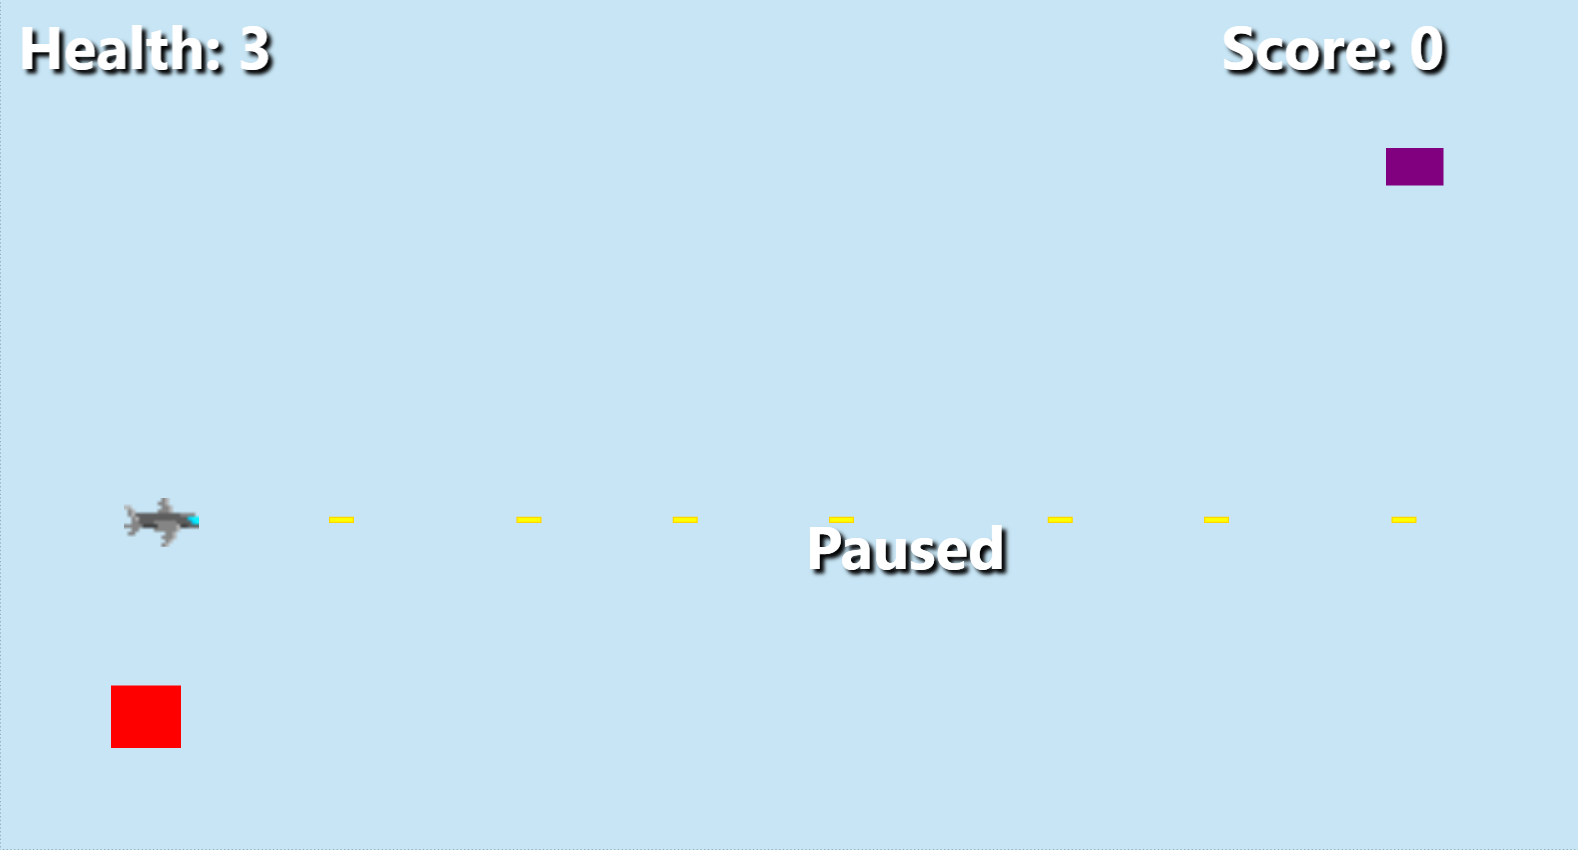
\includegraphics[height=250px, width=350px]{GAMEPAUSED.png}
\caption{This displays how the game looks when it is paused}
\label{gamepaused}
\end{figure}

\begin{figure}[ht!]
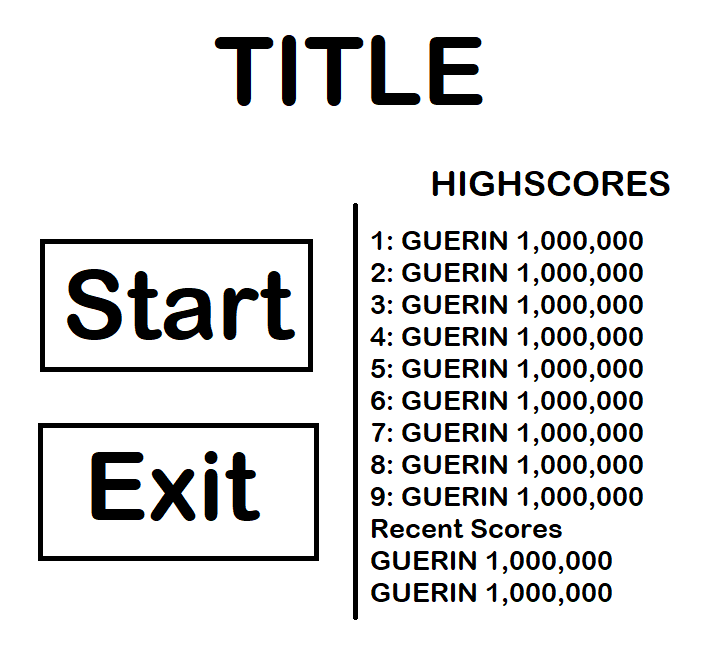
\includegraphics[height=250px, width=350px]{MOCKUP TITLE.png}
\caption{This displays an idea for how the menu screen will look}
\label{mockup}
\end{figure}

\begin{figure}[ht!]
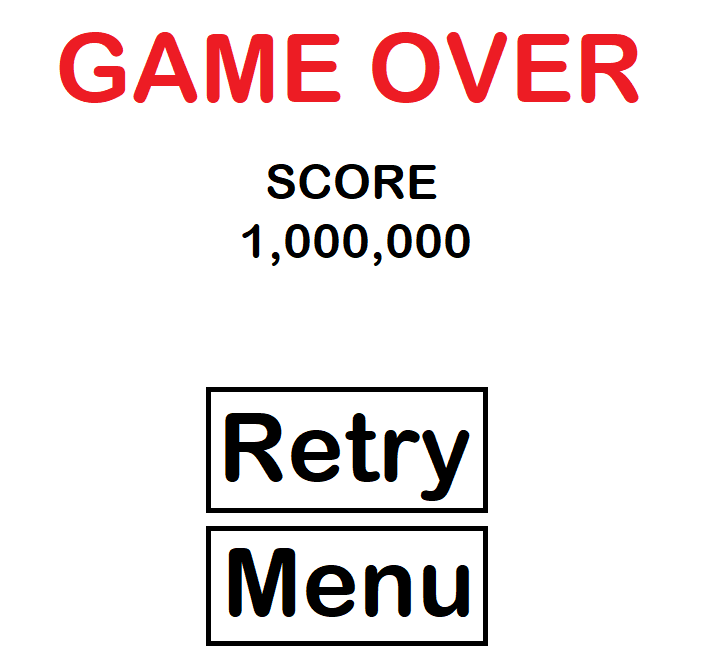
\includegraphics[height=250px, width=350px]{GAMEOVER MOCKUP.png}
\caption{This displays an idea for how the gameover screen will look}
\label{gameover}
\end{figure}

\begin{figure}[ht!]
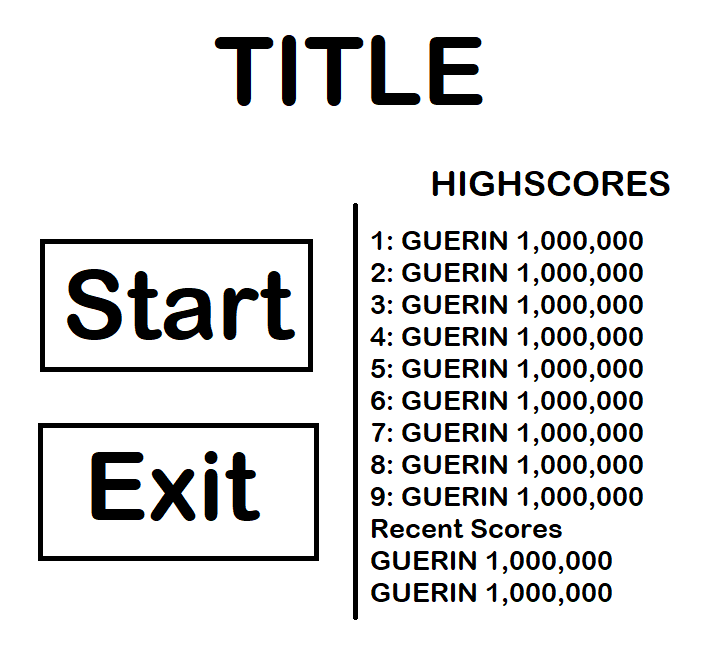
\includegraphics[height=250px, width=350px]{MOCKUP TITLE.png}
\caption{This displays an idea for how the menu screen will look}
\label{mockup}
\end{figure}


\section{Project Timeline}
We have already made a demoable prototype that we showed in class, but we have yet to develop the full featured product. The steps we took or will take to create the project will go as follows: 
\begin{enumerate}
\item We have made a game engine that will control several important functions such as: Movement control, enemy spawning, and collision detection.
\item We have made the movement controls and projectile firing. 
\item We have made the spawning of enemies and allow several different versions of enemies to be selected. This includes making an basic enemy object and its derrived children.
\item We have made the Pause Function
\item We will creare the system of collision detection. This also controls the losing of health and gaining of points as certain collisions are detected. 
\item We will create a Game Over state and display the appropriate state for a game over.
\item Will we reate a main menu with High Score Board.
\item We will polish Audio and Visual presentation.
\end{enumerate}

\subsection{Important Dates}
\begin{itemize}
\item4/28/22 - In class demo
\item4/29/22 - Final documentation for the semester
\end{itemize}

\section{Project Structure}
The project switches between three main windows, that open and close as appropriate. The Main Menu has the controls for starting and exiting the game as well as displaying the highest scores. The GameMain is what controls the game and is what the player will spend most of their time in. This window is switches to GameOverWindow upon the player losing the game. The GameOverWindow allows the player to go straight to either the GameMain or MainMenu window, as well as displaying the score the player just achieved. The game currently has three different sizes of enemies, each will reward more points like  targets (i.e. the smaller the target, the more points it is worth).


\subsection{UML Outline}
\ref {UML}
I'n this figure you can see the UML for our program. The meat of the program is in the GameEngine class, that contains several important functions that are called by both the game's main window GameMain and the GameOverWindow. The Bullet class is derived from the bullet template (Template Design Pattern) and provides the fireBullet function the Rectangle it needs to add to the screen. The spawnEnemy function needs an Enemy class, including EnemyBasic and it's two children (Factory Design Pattern). The three windows are designed to be swapped between when certain functions are called. The enemies use a Factory Design Pattern because the creational pattern is used to make different variants off of the basic enemy class. The bullet uses a Template Design Pattern because the bullet class is derived from an abstract template that could have multiple variations.
\begin{figure}[ht!]
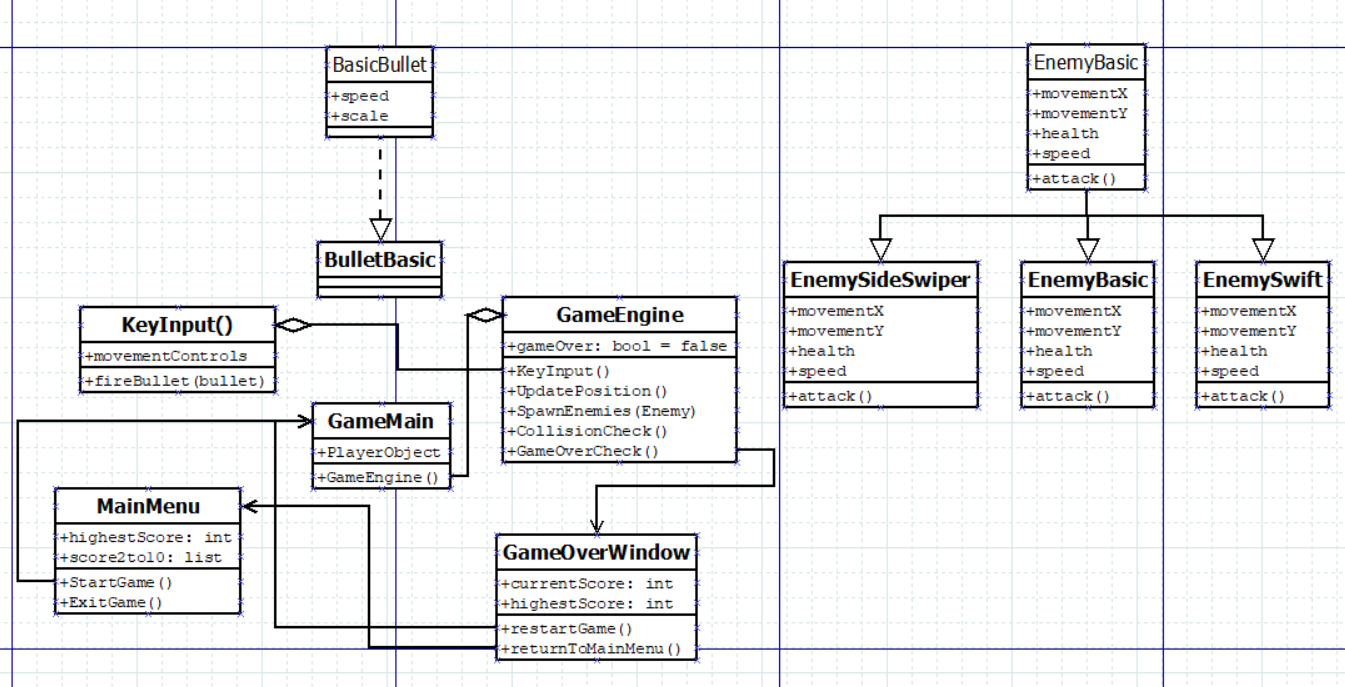
\includegraphics[height=250px, width=350px]{DIA.png}
\caption{This is the UML for Spitfire '91}
\label{UML}
\end{figure}

\subsection{Design Patterns Used}
We are implementing the Factory Pattern and Template Pattern for the project. You can see the factory pattern with the enemy classes, with two children of EnemyBasic being derived from EnemyBasic to create new enemy variants. Similarly, Template pattern is used by the bullet class. Although only one type of bullet was created for the project, it still derives from an abstract Template.


\section{Results}
Turns out WPF is not really meant for making games, and by not really, we mean not at all. We had to find weird workarounds and use things in strange unintended ways. We worked with the default WPF canvas. Currently we have a game where you can move around the plane and shoot, but not much else. As it currently stands, enemy spawning is working, but their collision detection isn't. Without enemy collison various game functions like health, scoring, and the game over have no function. We were able to put in music, because that ended up being much simpler to do than we thought it would be.

\subsection{Future Work}
We are about $\frac{2}{3}^{rds}$ done with the project, but we have run out of the time in the semester. Highest priority is getting collision detection to work, as without collision detection key functions of the game like scoring have no purpose or function. Once that is done we can move to making the Main Menu and Game Over menu, including the saving and displaying of high scores.





% that's all folks
\end{document}

